\setcounter{chapter}{1}

\chapter{数列极限与数值级数}

\section{数列极限}

\subsection{数列}

{\bf 教材P45:}按一定规律排列的无穷多个(相同或不相同的)数,记作:
$$a_1,a_2,\ldots,a_n,\ldots$$
或者$\{a_n\}$。

$\{a_n\}$的实质是定义在$\mathbb{N}_+$上的函数,即所谓的{\it 整标函数}\ps{教材上的说法是“可视为”},即
$$a_n:\mathbb{N}_+\to\mathbb{R}$$
也可以将其视为一个动点随$n$增大所留下的运动轨迹。

{\bf 命题:}一个集合是可数的,当且仅当它可以表示为一个数列。

{\bf 思考:}数列与集合有哪些区别?\ps{1、有序-无序;2、无限-可能有限;3、可重复-不可重复}

{\bf 例:}数列举例

\begin{enumerate}[(1)]
  \setlength{\itemindent}{1cm}
  \item[(1)] $\left\{\df{n+1}n\right\}:\df 21,\df 32,\df43,\df54,\df65,\ldots$
  \item[(2)] $\left\{\df{(-1)^n}n\right\}:-1,\df12,-\df13,\df14,-\df15,\df16,\ldots$
  \item[(3)] $\{n^2\}:1,4,9,16,25,36,\ldots$
  \item[(4)] $\left\{n^{(-1)^n}\right\}:1,2,\df13,4,\df15,6,\ldots$
\end{enumerate}

\subsection{数列的极限}

{\bf 极限:} 一种无限靠近的趋势 
	
\begin{enumerate}
  \setlength{\itemindent}{1cm}
  \item 对于数列而言,无限靠近的趋势意味着什么? 
  \item 如何从数学上严格表达这种趋势? 
\end{enumerate}

{\bf 定义2.1.2} 

对于数列$\{a_n\}$,若存在常数$a$,对于任意给定的正数$\e$,均存在正整数$N$,当$n>N$时,恒有
$$|a_n-a|<\e$$
成立,则称{\bf 数列$\{a_n\}$存在极限(或收敛)},常数$a$称为该数列的极限,记为
$$\lim_{n\to\infty}a_n=a$$
或
$$a_n\to a\;(n\to\infty)$$
若上述常数$a$不存在,则称数列$\{a_n\}$不存在极限(或{\bf 发散})。

\begin{center}
	\resizebox{!}{3cm}{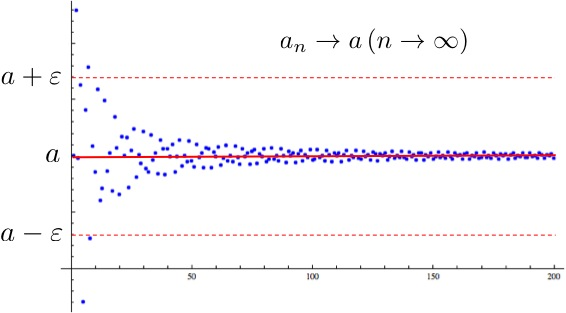
\includegraphics{./images/ch2/lim-en/en1.jpg}}\quad
	\resizebox{!}{3cm}{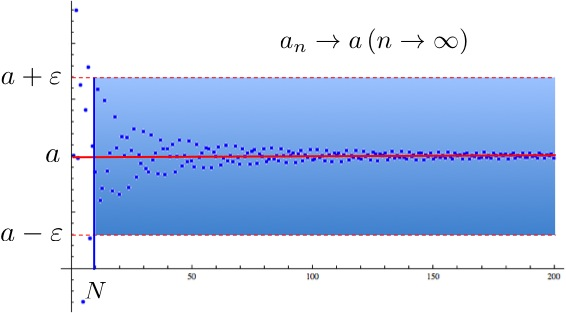
\includegraphics{./images/ch2/lim-en/en2.jpg}}
	
	\resizebox{!}{3cm}{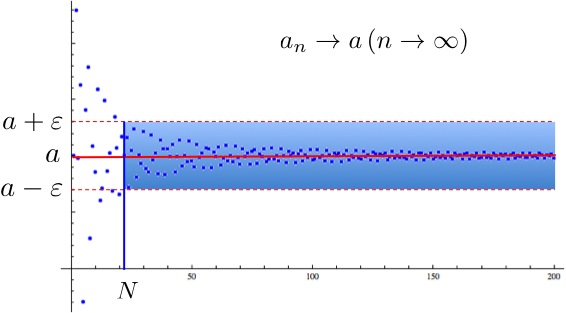
\includegraphics{./images/ch2/lim-en/en3.jpg}}\quad
	\resizebox{!}{3cm}{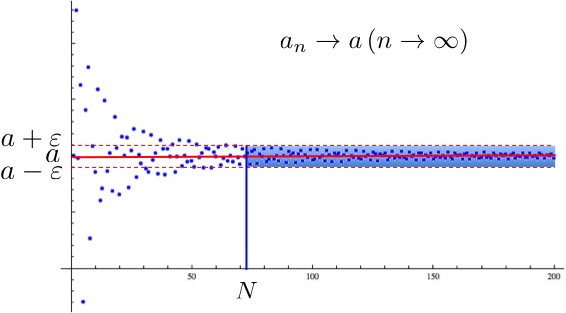
\includegraphics{./images/ch2/lim-en/en4.jpg}}
	
	\resizebox{!}{3cm}{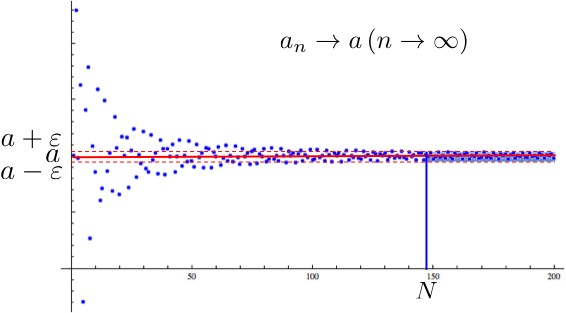
\includegraphics{./images/ch2/lim-en/en5.jpg}}
\end{center}

等价说法:

$$\lim_{n\to\infty}a_n=a\Leftrightarrow
\forall\e>0,\exists N\in\mathbb{Z}_+,\forall n>N,|a_n-a|<\e\eqno{(1)}$$

{\bf 讨论:}以下说法和$(1)$等价的是:

\begin{enumerate}
  \setlength{\itemindent}{1cm}
%   \item[(2)] $\forall\e>0$,$\exists N>0$,$\forall
%   n>N$,$|a_n-a|<\e$ \hfill{$\surd$}\\
%   \hfill(直接写$\exists N$即可)
  \item[(2)] $\forall\e>0$,$\exists N$,$\forall
  n>N$,$|a_n-a|\leq\e$ \hfill{$\surd$} 
  \item[(3)] $\exists N>0$,$\forall\e>0$,$\forall
  n>N$,$|a_n-a|<\e$ \hfill{$\times$} 
  \item[(4)] $\forall\e>0$,仅有有限多个$n$,使得$|a_n-a|\geq\e$
  \hfill{$\surd$} 
  \item[(5)] $\forall\e>0$,总有无穷多个$n$,使得$|a_n-a|<\e$
  \hfill{$\times$} 
  \item[(6)] $\forall\e>0$,要使$|a_n-a|<\e$,只须$n$充分大 \hfill{$\surd$}
  \item[(7)] $\forall\e>0,\exists N\in\mathbb{N}_+,\forall
  n>N,|a_n-a|<2\e$\hfill{$\surd$}
\end{enumerate}

{\bf 注:}

\begin{itemize}
  \setlength{\itemindent}{1cm}
  \item $a$是确定的数 ( {不能是$\pm\infty$}) 
  \item “$\forall\e>0$”应该理解为{“对任意小的$\e>0$”}
  \item $N$由$\{a_n\}$和$\e$共同决定, “存在$N$”可理解为{“存在充分大的$N(\e)$}”; 
   {如果$N$能够满足定义, 任意比$N$大的数都能够满足定义; 通常$\e$取得越小,
  $N$需要取得越大} \ps{$\{a_n\}$的收敛性与其任意多的有限项无关!!}
  \item 给定$C>0$,“$|a_n-a|<\e$” 可替换为{“$|a_n-a|<C\e$”}, 其中$C>0$为常数
\end{itemize}

{\bf 例:}证明:
$$\limn(-1)^n\df1{n^2}=0$$

{\bf 例:}证明:
$$\limn\left(\df n{n+1}\right)^2=1$$

{\bf 例:}证明:若$\limn a_n=a$,则$\limn|a_n|=|a|$

{\bf 例:}证明:若$|q|<1$,则$\{q^n\}$收敛。

{\bf 思考:}已知$|q|>1$时,$\{q^n\}$发散,请问该如何证明?

{\bf 注:}利用有界性,也可以证明发散。

\begin{shaded}
	{\bf 【极限定义的反面说法】}
	
	$$\limn a_n\neq a\Leftrightarrow\exists\e_0>0,\forall N>0,\exists
		n_0>N,|a_{n_0}-a|\geq\e_0$$
	
	{\bf 例:}证明:$\limn\df 1n\neq 1$
	
	{\bf P51,例5:}证明$\{(-1)^n\}$发散。 
	
	{\bf 注:}对比教材上的证明方法与用反面说法证明的区别。
	
	{\bf 思考:}数列发散可能有哪些不同的情形?(趋向无穷,或振荡)
	
\end{shaded}

\subsection{数列极限的基本性质}

\subsubsection{【唯一性】}

{\bf 定理2.1.1:}数列极限若存在,必唯一。\ps{唯一性的要求决定了当前的极限定义。
“记录重大技术突破的技术发展史其实就是一部人类社会发展的技术选择史”}

\begin{center}
	\resizebox{!}{4cm}{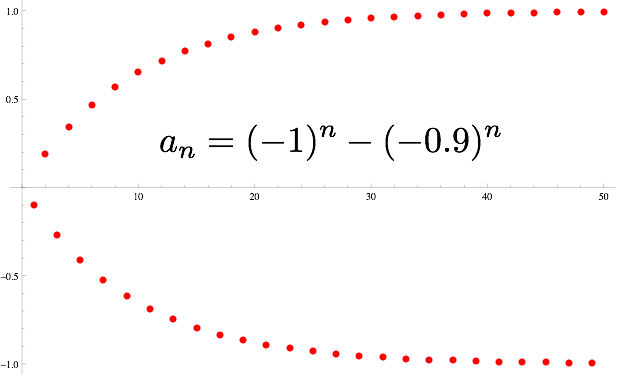
\includegraphics{./images/ch2/1-0.9n.jpg}}
\end{center}

{\bf 典型方法:}若对$\forall\e>0$,有$|a-b|<\e$,则$a=b$

\subsubsection{【有界性】}

{\bf 定理2.1.2:}数列$\{a_n\}$若收敛,则$\{a_n|n\in\mathbb{Z}_+\}$必有界。

\begin{center}
	\resizebox{!}{4cm}{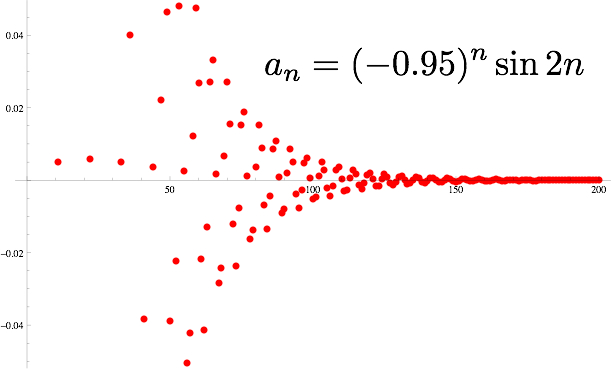
\includegraphics{./images/ch2/sin2nn.jpg}}
\end{center}

{\bf 典型方法:}利用$\e$的特定取值控制无穷的部分,剩余的有限集自然是有界的

{\bf 例:}讨论$\{\sqrt[n]{n!}\}$的敛散性。

{\bf hint:}注意到$\forall a>0$,当$n$充分大时,$n!>a^n$,故$\{\sqrt[n]{n!}\}$无界,
从而发散。

\subsubsection{【保号性】}

{\bf 定理2.1.3:}设$\lim\limits_{n\to\infty}a_n>0$,则$\exists N>0$,
		对$\forall n>N$,$a_n>0$
		
{{\bf 推论:}} 
\begin{enumerate}
  \setlength{\itemindent}{1cm}
  \item 设对$\forall n\in\mathbb{N}$,$a_n\geq
  0$, $\lim\limits_{n\to\infty}a_n=a$, 则$a\geq 0$ 
  \item 设$\lim\limits_{n\to\infty}a_n=a\ne
  0$, 则$\exists N$,当$n>N$时,$|a_n|>|a|/2$ 
  \item
  设$\lim\limits_{n\to\infty}a_n=a$, 且最多有有限个$a_n$小于零, 则$a\geq 0$
\end{enumerate}	

{\bf 注:}保号性的实质,是极限运算保持不等号的方向不变
$$a_n\geq b_n\,(n\in\mathbb{Z}_+)\Rightarrow\limn a_n\geq\limn b_n$$

\section{数列极限的性质与判敛}

\subsection{四则运算的性质}

{\bf 定理2.2.1:}\ps{强调:只对有限次的四则运算有效!!!}
设数列$\{a_n\},\{b_n\}$分别以$a,b(b\neq 0)$为极限,则
数列$\{a_n\pm b_n\},\{a_nb_n\},\left\{\df{a_n}{b_n}\right\}$均收敛,且
\begin{enumerate}
  \setlength{\itemindent}{1cm}
  \item $\limn(a_n\pm b_n)=a\pm b$
  \item $\limn a_nb_n=ab$
  \item $\limn\df{a_n}{b_n}=\df ab$
\end{enumerate}

{\bf 注:}极限运算和四则运算可以交换次序——前提是极限存在,且为有限次四则运算

{\bf 例:}
\begin{eqnarray*}
	1&=&\limn \underbrace{\left(\df 1n+\df 1n+\cdots+\df 1n\right)}_{n}\\
	&=&\underbrace{\limn\df1n+\limn\df1n+\cdots+\limn\df1n}_{n}\\
	&=&n\limn\df1n=0
\end{eqnarray*}
$n$落在了极限符号之外,显然错误!!

{\bf P58-例2:}计算极限
$$\limn\df{2n^6+3n^4-n+10}{n^6+n^4+1}$$

{\bf P58-例1:}设$\limn(a_n+b_n)=1$,$\limn(a_n-b_n)=3$,证明$\{a_n\},\{b_n\}$收敛,并求其值。

{\bf 例:}计算极限
$$\limn\df{\cos^n\theta-\sin^n\theta}{\cos^n\theta+\sin^n\theta}\quad
(0\leq\theta\leq\df{\pi}{2})$$

{\bf 例:}$|x|<1$,计算
$$\limn(1+x)(1+x^2)\ldots(1+x^{2^n})$$

{\bf 定理2.2.1':}初等函数运算可以和极限运算交换次序。

{\bf 例:}设$a_n>0(n\in\mathbb{N})$,$\limn a_n=a$,证明:
$$\limn\sqrt{a_n}=\sqrt a$$

{\bf hint:} 若$a=0$,对$\e^2$,取$N$即可。

{\bf Ex:}$\limn\left(\df12+\df3{2^2}+\ldots+\df{2n-1}{2^n}\right)$

[hint]: let $x_n=\df12+\df3{2^2}+\ldots+\df{2n-1}{2^n}$, then
$$\df12x_n=\df12\left(\df12+\df1{2^2}+\ldots+\df1{2^n}\right)
-\df{2n-1}{2^{n+1}}\to\df32\;(n\to\infty)$$

{\bf 例:}$|\lambda|<1$,计算$\limn(\lambda+2\lambda^2+\ldots+n\lambda^n)
=\df{\lambda}{(1-\lambda)^2}$ 

{\bf EX:} $\limn\left(\sqrt{n+3\sqrt n}-\sqrt{n-\sqrt{n}}\right)=2$

{\bf EX:} $\limn\left(1-\df1{2^2}\right)\left(1-\df1{3^2}\right)\ldots
\left(1-\df1{n^2}\right)=\df12$

{\bf EX:} $\limn\sin^2\left(\pi\sqrt{n^2+n}\right)$

{\bf EX:} $\limn\left(\df32\cdot\df54\cdots\df{2^n+1}{2^n}\right)
=\limn2\left(1-\df12\right)\left(1+\df12\right)\left(1+\df1{2^2}\right)
\ldots\left(1+\df1{2^n}\right)=2$

{\bf EX:} $\sqrt{x+\sqrt{x+\sqrt x}}-\sqrt x\to\df12,\;(n\to\infty)$

\subsection{子数列的收敛性}

{\bf 子数列:}

$$\{a_{n_k}\}:\,a_{n_1},a_{n_2},\ldots,a_{n_k},\ldots$$

{\bf 注:}$\{n_k\}$本质上是一个正整数构成的数列,
所以子数列可以视为两个数列的复合

{\bf 定理2.2.2:}数列收敛,当且仅当其任意子数列收敛,且极限相同。

即:对任意严格单调递增的正整数数列$\{n_k\}$,
$$\limn a_n=a\Leftrightarrow\lim_{k\to\infty}a_{n_k}=a$$
$\{a_{n_k}\}$收敛于$a$的定义: $\forall \e>0$, $\exists
{K}$, $\forall {k>K}$, 有 $$|a_{{{n_k}}}-a|<\e,$$
 记为\ps{强调$k$变化而不是$n$变化}
$$\lim\limits_{{k\to\infty}}a_{n_k}=a\quad \mbox{或}\quad a_{n_k}\to
a\;{(k\to\infty)}$$

{\bf 推论:}若某个数列存在不收敛的子列,或者存在两个极限不相同的子列,则该数列不收敛。

{\bf 例P60,例4:}证明数列$\left\{n^{(-1)^n}\right\}$发散。

{\bf EX:} prove $\{\left(1+\df1{\sqrt n}\right)\sin\df{\pi\sqrt n}2\}$
divergence.

{\bf 定理2.2.3}(拉链定理)数列$\{a_n\}$收敛,当且仅当$\{a_{2n}\}$
和$\{a_{2n-1}\}$收敛于相同的极限。

{\bf 推论:}数列$\{a_n\}$收敛,当且仅当$\{a_{3n}\}$,$\{a_{3n+1}\}$和
$\{a_{3n+2}\}$收敛于相同的极限。

{\bf 注:}更一般性的推广:如果选择的子列能够完全覆盖原数列,或最多不能覆盖原数列中
有限多个数,且这些子列均收敛于相同的极限,则原数列收敛。

\subsection{夹逼(迫敛)定理}

{\bf 定理2.2.4:}设对任意$n\in\mathbb{N}$,$x_n\le a_n\le y_n$,
且$\{x_n\},\{y_n\}$收敛于相同的极限$a$,则$\limn a_n=a$。

\begin{center}
	\resizebox{!}{5cm}{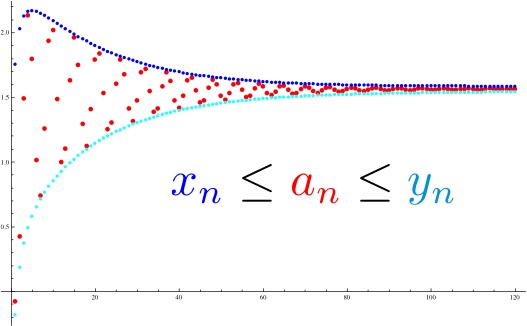
\includegraphics{./images/ch2/xay_n.jpg}}
\end{center}

{\bf P61,例5:}证明$\limn [(n+1)^k-{n}^k]=0$,其中$0<k<1$。

{\bf hint:}$n^k\left[\left(1+\df1n\right)^k-1\right]
<n^k\left(1+\df1n-1\right)=n^{k-1}\to 0\;(n\to\infty)$

{\bf P61,例6:}设$a>0$为常数,证明$\limn \sqrt[n]{a}=1$。

{\bf EX:} $\limn\df{\sqrt{n+\sqrt n}-\sqrt n}{\sqrt[n]{3^n+5^n+7^n}}=\df1{14}$

{\bf EX:} $\limn\sqrt[n]{n^5+5^n}=5$

{\bf EX:} given $\limn a_n=A$,
\begin{enumerate}
  \item $\limn\df{[na_n]}n=A$
  \item if $\lambda\in(0,1)$, compute
  $$\limn(a_n+\lambda a_{n-1}+\lambda^2a_{n-2}+\ldots+\lambda^na_0)=\df
  A{1-\lambda}$$
\end{enumerate}

{\bf EX:} $x\geq 0$, then
$$\limn\sqrt[n]{1+x^n+\left(\df{x^2}2\right)^n}=
\left\{\begin{array}{ll}
1&x\in[0,1]\\ x & x\in(1,2]\\ \frac{x^2}2& x>2
\end{array}\right.$$

{\bf EX:} $\limn\left(\df1{n+1}+\df1{\sqrt{n^2+1}}+\ldots
+\df1{\sqrt[n]{n^2+1}}\right)=1$

\subsection{单调有界原理}

{\bf 定理2.2.5:}单调有界的数列必收敛。\ps{只要数列从某一项开始单调即可!!!}

{\bf 【重要极限】}(P63-例7)
$$a_n=\left(1+\df{1}{n}\right)^n\to e\quad (n\to\infty)$$

{\bf 注:}需要掌握的重要性质
\begin{itemize}
  \setlength{\itemindent}{1cm}
  \item 数列$\left\{\left(1+\df 1n\right)^n\right\}$严格单调递增有上界
  \item 数列$\left\{\left(1+\df 1n\right)^{n+1}\right\}$严格单调递减有下界
  \item 显然,二者极限相同
\end{itemize}

\begin{shaded}
	{\bf 关于Napier常数$e$}
	
	{\bf 例:}若将$a>0$分成若干份,使得总乘积最大,由平均值不等式可知,显然
	等分最有利,但该分成多大的一份呢?分析可证明分成最接近于$e$的大小最合适。
	
	{\bf 例:}$\e_n=e-\sum\limits_{k=0}^n\df1{k!}$,则
	$$\limn\e_n(n+1)!=1$$
	
	[hint]:利用$\df00$型的Stolz定理
	
	{\bf 例:}$\delta_n=e-\left(1+\df1n\right)^n
	<\left(1+\df1n\right)^{n+1}-\left(1+\df1n\right)^n
	=\left(1+\df1n\right)^n\df1n<\df en<\df3n$
	
	事实上,$\limn\df{2n\delta_n}e=1$
	
	{\bf 重要不等式:}由$\left(1+\df1n\right)^n<e<\left(1+\df1n\right)^{n+1}$,
	可得
	$$\df1{n+1}<\ln\left(1+\df1n\right)<\df1n$$
	{\bf Eular常数:}
	$$\gamma=\limn\left(\sumn\df1k-\ln n\right)\approx 0.5772\ldots$$
\end{shaded}

{\bf 例:}证明$\a_n=\df1{n+1}+\ldots+\df1{2n},\;(n\in\mathbb{Z}_+)$收敛。

[hint]:利用$\df1{n+1}<\ln\left(1+\df1n\right)<\df1n$,极限为$\ln2$

\subsection{递推数列的判敛}

{\bf 例:}已知$a_1,a_2$为常数,数列$\{a_n\}$满足:
$$a_n=\df 12({a_{n-1}+a_{n-2}})\quad(n>2).$$
证明$\{a_n\}$收敛,并求其极限。

\begin{shaded}
	{\bf 特征根法求解求解二阶常系数齐次递推}
	
	$$a_{n+2}=Aa_{n+1}+Ba_n\,(AB\ne 0, A+B\ne 1)$$
	特征方程为:
	$$r^2=Ar+B$$
	\begin{enumerate}[(1)]
	  \setlength{\itemindent}{1cm}
	  \item 若特征方程有相异实根$p,q$,则
	  $$a_n=C_1p^n+C_2q^n$$
	  其中系数$C_1,C_2$由方程
	  $$\left\{\begin{array}{l}
	  a_1=C_1p+C_2q\\
	  a_2=C_1p^2+C_2q^2
	  \end{array}\right.$$
	  可解得
	  $$C_1=\df{a_1q-a_2}{p(q-p)},\quad 
	  C_2=\df{a_1p-a_2}{q(p-q)}$$
	  \item 若有两个相等的实根$r$,则
	  $$a_n=[C_1r+C_2(n-1)]r^{n-1}$$
	  与(1)类似地可求出系数$C_1,C_2$
	\end{enumerate}
	
	{\bf 例:}Fibonacci数列:$a_{n+2}=a_n+a_{n+1}$
	
	$$a_n=\df1{\sqrt5}\left(\df{1+\sqrt5}2\right)^{n+1}
	-\left(\df{1-\sqrt5}2\right)^{n+1}$$
	
\end{shaded}

{\bf P53-例9:}设$a_1>0$,$a_{n+1}=\df 12\left(a_n+\df 1{a_n}\right)\,
(n=1,2,\ldots)$,证明$\{a_n\}$收敛,并求其极限。

{\bf 注:}
\begin{itemize}
  \setlength{\itemindent}{1cm}
  \item 递推式两边同时取极限,解方程求得极限的值,是最便利的计算递推数列极限的方法
  \item 若通过以上方法可以求出极限的值,通常只需证明数列单调有界即可
  \item 若该方法无法求得极限的值,则只能利用递推式推导数列通项,进而证明其收敛并计算极限
\end{itemize}

{\bf 例:}计算下列极限
\begin{enumerate}[(1)]
  \setlength{\itemindent}{1cm}
  \item $\limn\df{n^2}{a^n}\quad (a>1)$
  \item $\limn\df{n!}{n^n}$
  \item $\limn\underbrace{\sqrt{c+\sqrt{c+\ldots+\sqrt{c}}}}_{n\mbox{\small
		  个根号}}$
\end{enumerate}

{\bf }若极限存在,可由通项公式反推递推式,然后两边取极限,解方程求得极限值

{\bf 例:}$x_1=\df c2$,$x_{n+1}=\df c2+\df{x_n^2}2\,(n\in\mathbb{Z}_+)$,
证明:若$c>1$,则$\{x_n\}$发散。

[hint]: 设极限为$A$,则$A^2-2A+c=0$,$c>1$时,无解,必发散。

{\bf 例:}$a_0>b_0>0$,
$$a_n=\df12(a_{n-1}+b_{n-1}),\quad
b_n=\sqrt{a_{n-1}b_{n-1}}\;(n\in\mathbb{Z}_+)$$
证明:$\{a_n\},\{b_n\}$收敛于同一极限。

[hint]:$b_0<b_1<a_1<a_0$,利用数学归纳法证明:
$$b_0<b_1<\ldots<b_n<a_n<\ldots<a_1<a_0$$

{\bf 例:}证明:$a_n=\sqrt{1+\sqrt{2+\ldots+\sqrt{n}}}$收敛。

[hint]: we hvae
$$\sqrt{n-1+\sqrt n}<\sqrt{n-1+2\sqrt{n-1}+1}=\sqrt{n-1}+1,$$
and hence by using $\sqrt{n-1}<2\sqrt{n-2}$ iteratively

{\bf Ex:} Given $x\in(0,3),\; x_{n+1}=\sqrt{x_m(3-x_n)},\;(n\in\mathbb{Z}_+)$,
prove $\{x_n\}$ convergence, and find its limit.

[hint]: $0<x_2\leq\df12[x_1+(3-x_1)]=\df32$, then by induction, we find
$0<x_n\leq\df32$. On the other hand,
$$x_{n+1}-x_n=\df{\sqrt{x_n}(3-2x_n)}{\sqrt{x_n(3-x_n)}+\sqrt{x_n}}\geq 0.$$

\subsection{Stolz定理}

{Stolz定理}($\df{\infty}{\infty}$形式)

设数列$\{y_n\}$满足$\limn\df 1{y_n}=0$,且$\{y_n\}$至少从某一项开始保持严格单调递增,
则对任意数列$\{x_n\}$,若$\limn\df{x_n-x_{n-1}}{y_n-y_{n-1}}$存在,则必有
$$\limn\df{x_n}{y_n}=\limn\df{x_n-x_{n-1}}{y_n-y_{n-1}}$$

{\bf 注:}Stolz定理主要用于计算"$\df{\infty}{\infty}$型"的极限

{\bf 推论}(Cauchy极限定理)若$\{a_n\}$收敛,则
$$\limn\df{a_1+a_2+\ldots+a_n}n=\limn a_n$$

{\bf 例:}计算以下极限
\begin{enumerate}[(1)]
  \setlength{\itemindent}{1cm}
  \item $\limn\df{1+\sqrt 2+\sqrt[3]{3}+\ldots+\sqrt[n]{n}}{n}$ 
  \item $\limn\df{1^k+2^k+\ldots+n^k}{n^{k+1}},\quad(k\in\mathbb{N})$ 
  \item $\limn\left(\df{1^k+2^k+\ldots+n^k}{n^{k}}-\df
  n{k+1}\right),\quad(k\in\mathbb{N})$\\
  {\bf 提示:}(3)
  \begin{eqnarray*}
  	\mbox{原式}&=&\limn\df{(k+1)(1^k+2^k+\cdots+n^k)-n^{k+1}}{n^k(k+1)}\\
  	&=&\limn\df{(k+1)(n+1)^k-[(n+1)^{k+1}-n^{k+1}]}{(k+1)[(n+1)^k-n^k]}\\
  	&=&\limn\df{(k+1)[n^k+kn^{k-1}+P_{k-2}^{(1)}(n)]
  	-\left[(n+1)^k+(n+1)^{k-1}n+\cdots+n^k\right]}{(k+1)
  	\left[(n+1)^{k-1}+(n+1)^{k-2}n+\cdots+n^{k-1}\right]}\\
  	&=&\limn\df{(k+1)[n^k+kn^{k-1}+P_{k-2}^{(1)}(n)]-(k+1)n^k
  	-\df{k(k+1)}2n^{k-1}-P_{k-2}^{(2)}(n)}
  	{(k+1)\left[\df{k(k+1)}{2}n^{k-1}+P_{k-2}^{(3)}(n)\right]}\\
  	&=&\df12
  \end{eqnarray*}
\end{enumerate}

{\bf 推论:}设$\{a_n\}$为正数列,则
$$\limn\sqrt[n]{a_1a_2\ldots a_n}=\limn a_n$$

{\bf 推论:}设$\{a_n\}$为正数列,$\limn\df{a_{n+1}}{a_n}=q$,
则$\limn\sqrt[n]{a_n}=q$

[提示]:设$b_1=a_1,\;b_n=\df{a_n}{a_{n-1}}$,利用上一推论即可。

{\bf 例:}计算极限$\limn\df{n!2^n}{n^n}$

{\bf 例:}计算$\limn\df{1!+2!+\ldots+n!}{n!}$

{\bf 定理}($\df00$型)设$\limn a_n=\limn b_n=0$,且$\{a_n\}$严格
单调递减,若$\limn\df{b_{n+1}-b_n}{a_{n+1}-a_n}=l$($l$可以为$\pm\infty$),
则$\limn\df{b_n}{a_n}=l$

[hint]:证明中用到如下不等式:若
$$\df{p_i}{q_i}\in(a,b)\;(q_i>0,i=1,2,\ldots,n,)$$
则
$$\df{\sum\limits_{i=1}^np_i}{\sum\limits_{i=1}^nq_i}\in(a,b)$$

{\bf 例:}设$\limn a_n=\alpha,\limn b_n=\beta$,则
$$\limn\df{a_1b_n+a_2b_{n-1}+\ldots+a_nb_1}n=\alpha\beta$$

{\bf 例:}计算$\limn\df{\ln n}{1+\frac12+\ldots+\frac1n}$

{\bf EX:} if $\limn a_n=A$, then
\begin{enumerate}[(1)]
  \setlength{\itemindent}{1cm}
  \item $\limn\df{a_0+a_1+\ldots+na_n}{n^2}=\df a2$
  \item $\limn\df{a_1+\frac12a_2+\ldots\frac1na_n}{\ln n}=a$
\end{enumerate}

{\bf Q:} if $\limn x_n=a$, wether $\limn\df{x_{n+1}}{x_n}$ exists?

A: not for sure, as we have $x_n=\df1{3^{[\frac{n+1}2]}}$ (it is
$\df13, \df13, \df 1{3^2}, \df1{3^2}, \df1{3^3}, \df1{3^3},\ldots$ )


\section{数值级数}

{\bf 级数(无穷和):}无穷多个数按照一定次序求和
$$\sum\limits_{k=1}^{\infty}a_k
=\lim_{n\to\infty}\left(\sum_{k=1}^na_k\right)$$  
其中$a_k\in\mathbb{R}\,(k\in\mathbb{N})$。

\begin{itemize}
  \item {\bf 部分和(数列):}$S_n=\sum\limits_{k=1}^na_k$
  \item {\bf 级数收敛}$\Leftrightarrow\{S_n\}$收敛
\end{itemize}

{\bf 例:}判断下列级数的收敛性
\begin{enumerate}[(1)]
  \setlength{\itemindent}{1cm}
  \item $\sumn q^n\quad (q>0)$ (\ldots\ldots 几何级数) 
  \item $\sumn\df{1}{n(n+1)}$ 
  \item $\sumn\df 1n$ (\ldots\ldots 调和级数) 
% 		  \item $\sumn\df 1n^2$
  \item $\sumn (-1)^n$
\end{enumerate}

\begin{shaded}
{\bf 【关于调和级数】}

调和级数发散的速度慢得让人有些不可思议,调和级数的前$1000$项的和约为$7.485$,
前$100$万项的和约为$14.357$,前$10$亿项的和约为$21$,前一万亿项和约为$28$,
当它的和超过$100$时,如果每一项在纸带上只占$1$毫米,我们必须使用$10^{43}$毫米长
的纸带,这大约是$10^{25}$光年,而宇宙估计尺寸只有$10^{12}$光年,因此也难怪大家都会认为它是收敛的。

{\bf 【Eular常数】}

{\it Eular常数最先由瑞士数学家莱昂哈德·欧拉(Leonhard Euler)
在1735年发表的文章 De Progressionibus harmonicus observationes 中定义。
欧拉曾经使用C作为它的符号,并计算出了它的前6位小数。1761年他又将该值计算到了16位小数。}
$$\gamma=\limn\left[\sum\limits_{k=1}^n\df1k-\ln n\right]
=\int_1^{\infty}\left(\df1{[x]}-\df1x\right)\d x$$
由不等式$\ln(1+x)<x,(x\in(-1,+\infty),x\ne 0)$,
$$S_n=\sum\limits_{k=1}^n\df1k-\ln n>\sum\limits_{k=1}^n
\ln\left(1+\df1k\right)-\ln n=\ln(n+1)-\ln n>0.$$
$$S_n-S_{n+1}=\ln(n+1)-\ln n-\df1{n+1}>-\left(-\df1{n+1}\right)
-\df1{n+1}=0.$$
由单调有界原理可知$\{S_n\}$收敛。
\end{shaded}

\subsection{收敛级数的性质}

\begin{enumerate}[{\bf 【性质1】}]
  \item {\bf 定理2.3.1}(级数收敛的必要条件) 
  $$\sumn a_n\mbox{收敛}\Rightarrow\limn a_n=0$$
  \item $\sumn
  a_n$收敛$\Leftrightarrow\sum\limits_{n=k}^{\infty}a_n$收敛$(k\in\mathbb{N})$
  \ps{讨论收敛性时只需考虑部分和的后一部分,因为数列的收敛性与其前任意项无关}
  \item {\bf P59-例2:}$\{a_n\}$收敛$\Leftrightarrow\sumn(a_{n+1}-a_n)$收敛
  \item {\bf 定理2.3.2-3:}两个收敛级数的线性组合仍然收敛  
  \item {\bf 定理2.3.4:}增加、减少或改变级数中的有限项不影响其敛散性  
  \begin{itemize}
    \item {{增减或改变数列中的有限项不改变其敛散性}} 
  \end{itemize}
  \item {\bf 定理2.3.5:}若$\sumn a_n$收敛,不改变求和顺序,
  任意合并其中的项,所得新的级数仍收敛 
  \begin{itemize}
    \item {\bf 推论:}合并收敛级数中的相邻项,所得级数仍收敛 
    \item {{对发散级数,该性质不成立}} 
    \item {{改变求和次序,可能改变级数的收敛和}},例:$\sumn\df{(-1)^n}n$
  \end{itemize}
  \item (Cauchy原理)级数$\sumn a_n$收敛当且仅当:$\forall\e$,
  $\exists N\in\mathbb{Z}$,使对$\forall n>N$和$\forall p\in\mathbb{Z}^+$,
  都有
  $$|a_{n+1}+a_{n+2}+\ldots+a_{n+p}|<\e.$$
\end{enumerate}

{\bf 例:}判断以下级数的敛散性;若收敛,求其和

\begin{enumerate}[(1)]
  \setlength{\itemindent}{1cm}
  \item $\sumn\ln\left(1+\df 1n\right)$
  \item
  $\sumn\left[\prod\limits_{k=0}^p(\alpha+n+k)\right]^{-1},\;(p\in\mathbb{N})$
  \item $\sumn\df{x^{2^{n-1}}}{1-x^{2n}}$
  \item $\sumn\df{1}{\sqrt n}$
\end{enumerate}

{\bf 例:}利用Cauchy原理证明$\sumn\df1{n^2}$收敛

\begin{align}
	&|a_{n+1}+a_{n+2}+\ldots+a_{n+p}|\notag\\
	&<\df1{(n+1)(n+2)}+\df1{(n+2)(n+3)}+\ldots+\df1{(n+p-1)(n+p)}\notag\\
	&=\df1n-\df1{n+p}<\df1n\notag
\end{align}

{\bf 注:}直接使用比较判别法证明更为简洁

{\bf EX:} Which is true?
\begin{enumerate}[(1)]
  \setlength{\itemindent}{1cm}
  \item $\{a_n\}$ and $\sumn a_n$ converge at the same time
  \item $k\ne 0$, then $\sumn a_n$ and $\sumn ka_n$ converge at
  the same time
  \item $\sumn a_n$ converge, $\sumn b_n$ diverge, then
  $\sumn(a_n+b_n)$ diverge
  \item $\sumn a_n$ and $\sumn b_n$ both diverge, then 
  $\sumn(a_n+b_n)$ diverge
  \item if $\sum\limits_{n=1}^{\infty}a_{2n}$ and
  $\sum\limits_{n=1}^{\infty}a_{2n-1}$ both converge, then
  $\sumn a_n$ converge
  \item if $\sum\limits_{n=1}^{\infty}(a_{2n}+a_{2n-1})$, then
  $\sumn a_n$ converge
\end{enumerate}

{\bf EX:} find the sum
\begin{enumerate}[(1)]
  \setlength{\itemindent}{1cm}
  \item $\sumn\df1{n(n+1)(n+2)}=\df14$
  \item $\sumn\sin\df{\pi}6$ diverge, so it doesn't exist
\end{enumerate}

{\bf EX:} $\sumn\df{n}{3^n}$

[hint]: 1) denote $S_n=\df13+\df2{3^2}+\ldots+\df n{3^n}$, then
$$\df13S_n=\left(\df1{3^2}+\df2{3^2}+\ldots
+\df{n-1}{3^n}\right)+\df{n}{3^{n+1}}$$
hence
$$\df23S_n=\df12\left(1-\df1{3^n}\right)-\df{n}{3^{n+1}}\to\df12
(n\to\infty)$$

2) for $n<2^n$, we have $\df{n}{3^n}<\left(\df23\right)^n$

3) ration test

4) root test

\section{同号级数的收敛性}

\subsection{同号级数收敛的充要条件}

{\bf 定理2.4.1:}正项级数收敛,当且仅当其部分和数列有界。

{\bf P64-例1:}证明$\sumn\df1{n!}$收敛。

\subsection{比较判别法}

{\bf 定理2.4.2}(比较判别法的不等式形式)若对充分大的$n$,总有$0\leq a_n\leq b_n$,则
\begin{enumerate}
  \setlength{\itemindent}{1cm}
  \item 若$\sumn b_n$收敛,则$\sumn a_n$收敛
  \item 若$\sumn a_n$发散,则$\sumn b_n$发散
\end{enumerate}

{\bf P66-例3:}证明:\ps{p-级数}
\begin{enumerate}[(1)]
  \setlength{\itemindent}{1cm}
  \item[(1)] $p>1$时,$\sumn\df1{n^p}$收敛;
  \item[(2)] $0<p\leq 1$时,$\sumn\df1{n^p}$发散。
\end{enumerate}

{\bf 【hint】:}(2),$p=1$时,显然发散。又因为
$$0<\df 1n<\df 1{n^p},\quad (0<p<1),$$
已知调和级数发散,故p-级数发散;

(1)由以下推导可知$p>1$时,p-级数的部分和数列有界
\begin{eqnarray*}
	S_{(2^k)^p}&=&1+\df 1{2^p}+\underbrace{\left(\df1{3^p}+\df1{(2^2)^p}\right)}_2
				+\underbrace{\left(\df1{5^p}+\ldots+\df1{(2^3)^p}\right)}_{2^2}+\ldots\\
				&&+\underbrace{\left[\df1{(2^{k-1}+1)^p}+\ldots+\df1{(2^k)^p}\right]}_{2^{k-1}}\\
			  &\leq &1+\df 1{2^p}+2\cdot\df1{2^p}+2^2\cdot\df1{(2^2)^p}
			    +\ldots+2^{k-1}\cdot\df1{(2^{k-1})^p}\\
			  &=&1+\df 1{2^p}+\left[\df1{2^{p-1}}+\left(\df1{2^{p-1}}\right)^2+
			    \ldots+\left(\df1{2^{p-1}}\right)^{k-1}\right]\\
			  &=&1+\df 1{2^p}+\df1{2^{p-1}}\df{1-\left(\df1{2^{p-1}}\right)
			    ^{k-1}}{1-\df1{2^{p-1}}}<1+\df 1{2^p}+\df1{2^{p-1}-1}
\end{eqnarray*}

{\bf 例:}讨论下列级数的敛散性
\begin{enumerate}[(1)]
  \setlength{\itemindent}{1cm}
  \item[(1)] $\sumn\df{1}{3^{\ln n}}$
  \hfill({[hint]:$a^{\ln b}=b^{\ln a},\;(a,b>0)$})
  \item[(2)] $\sum\limits_{n=2}^{\infty}\df 1{(\ln n)^{\ln n}}$
  \item[(3)] $\sum\limits_{n=3}^{\infty}\df 1{(\ln n)^{\ln\ln n}}$
  
  ([hint]: $\sum\limits_{n=3}^{\infty}\df 1{(\ln n)^{\ln\ln n}}=
  \sum\limits_{n=3}^{\infty}\df 1{e^{(\ln\ln
  n)^2}}>\sum\limits_{n=3}^{\infty}\df 1n,e.g. (\ln\ln n)^2<\ln n,e.g. \ln
  n<\sqrt{n}$)
\end{enumerate}

{\bf Note:} if $\e>0, a>1$, then with sufficient large $n$, we have
$$\ln n<<n^{\e}<<a^n<<n!<<n^n$$

{\bf EX:} with sufficient large $x$, $e^x>2x^4$, then with 
sufficient large $n$, we have $e^{\sqrt[3]n}>2n^{\frac 43}$, so
$\sumn e^{-\sqrt[3]n}$ converge

{\bf P66-例4:}设$a_n\leq c_n\leq b_n\;(n\in\mathbb{N})$,$\sumn a_n,\sumn b_n$均收敛,
则$\sumn c_n$收敛。
\begin{itemize}
  \setlength{\itemindent}{1cm}
  \item 类似于数列收敛的“夹逼定理”
  \item 不要求必须是正项级数
\end{itemize}

{\bf 推论}(定理2.5.2)若级数$\sumn|a_n|$收敛,则$\sumn a_n$也收敛。

{\bf 定理2.4.3}(比较判别法的极限形式)

已知$a_n,b_n$均非负$(n\in\mathbb{Z}_+)$,且$\limn\df{a_n}{b_n}=l$,则 
\begin{enumerate}
  \setlength{\itemindent}{1cm}
  \item 若$0<l<+\infty$,$\sumn a_n,\sumn b_n$同敛散 
  \item 若$l=0$,$\sumn b_n$收敛$\Rightarrow\sumn a_n$收敛 
  \item 若$l=+\infty$,$\sumn a_n$收敛$\Rightarrow\sumn b_n$收敛
\end{enumerate}

{\bf P67-例5-6:}判断以下级数的收敛性
\begin{enumerate}[(1)]
  \setlength{\itemindent}{1cm}
  \item $\sumn\df 1{2^n}\df{n^2+1}{2n^2-1}$ 
  \item $\sumn\df{n+1}{n^k+2}\quad (k=1,2,\ldots)$ 
  \item $\sumn\df{1}{n\sqrt[n]{n}}$ 
  \item $\sumn\df{1}{1+x^n}\quad(x>0)$
\end{enumerate}

{\bf 推论}(p-判别法)
设$a_n\geq 0\;(n=1,2,\ldots)$,则 
\begin{enumerate}
  \setlength{\itemindent}{1cm}
  \item 若存在$p>1$,使得$\limn n^pa_n$存在,则$\sumn a_n$收敛 
  \item 若$0<p\leq 1$,使得$\limn n^pa_n>0$,则$\sumn a_n$发散
\end{enumerate}

{\bf 例:}判断以下级数的收敛性
\begin{enumerate}[(1)]
  \setlength{\itemindent}{1cm}
  \item $\sumn\df{\arctan n}{n^{3/2}}$
  \item $\sumn\df{\ln n}{n^{5/4}}$\ps{任何正幂次函数的增长速度最终都比任意对数函数快}
\end{enumerate}

{\bf 推论:}$\sumn a_n$、$\sumn b_n$均为正项级数,若对充分大的$n$,总有
$$\df{a_{n+1}}{a_n}\leq\df{b_{n+1}}{b_n},$$
则若$\sumn b_n$收敛,$\sumn a_n$收敛。

{\bf 【hint】:}
$$a_{n+1}\leq\df{a_1}{b_1}b_{n+1}$$

{\bf 例:}讨论级数$\sumn\df{n^n}{t^nn!}$的敛散性。

{\bf 【hint】:}
$$\df{a_{n+1}}{a_n}=\df{\left(1+\df1n\right)^n}{t}\to\df et$$
when $t=e$, 
$$\df{a_{n+1}}{a_n}=e\left(\df n{n+1}\right)^n>1,$$
so $\limn a_n\ne 0$, so $\sumn a_n$ diverge.

{\bf 课后思考}(2012年全国大学生数学竞赛)
$\sumn a_n$和$\sumn b_n$均为正项级数,证明:
\begin{enumerate}
  \setlength{\itemindent}{1cm}
  \item 若$\limn\left(\df{a_n}{a_{n+1}b_n}-\df 1{b_{n+1}}\right)>0$,
  则$\sumn a_n$收敛;
  \item 若$\limn\left(\df{a_n}{a_{n+1}b_n}-\df 1{b_{n+1}}\right)<0$,
  且$\sumn b_n$发散,则$\sumn a_n$发散。
\end{enumerate}

[hint]:1)由已知,存在$q>0$和$N\in\mathbb{Z}_+$,对任意$n\geq N$,有
$$\df{a_n}{a_{n+1}b_n}-\df 1{b_{n+1}}>q,$$
从而
$$a_{n+1}<\df1q\left(\df{a_n}{b_n}-\df{a_{n+1}}{b_{n+1}}\right).$$
利用递推关系可得
$$\sum\limits_{k=N}^na_k<a_N+\df1q\left(\df{a_N}{b_N}-\df{a_n}{b_n}\right)
<a_N+\df1q\df{a_N}{b_N},$$
故$\sumn a_n$部分和有界,从而收敛。

{\bf 牢记:比较判别法仅对同号级数有效!!!}

{\bf EX:} $\sumn\left(\cot\df{n\pi}{4n-2}-\sin\df{n\pi}{2n+1}\right)$

[hint]: consider $\sumn\left(1-\cot\df{n\pi}{4n-2}\right)$ and
$\sumn\left(1-\sin\df{n\pi}{2n+1}\right)$. for
$$\limn\df{1-\sin\df{n\pi}{2n+1}}{\df1n}=\df{\pi}4$$
$$\limn\df{1-\sin\df{n\pi}{2n+1}}{\df1{n^2}}=\df{\pi^2}{32}$$

\subsection{比值判别法}

{\bf 定理2.4.4}(d'Alembert判别法)
设$a_n\geq 0(n=1,2,\ldots)$,$\limn\df{a_{n+1}}{a_n}=q$,则
\ps{极限形式} 
\begin{enumerate}
  \setlength{\itemindent}{1cm}
  \item $0\leq q<1\Rightarrow\sumn a_n$收敛 
  \item $q>1\Rightarrow\sumn a_n$发散
\end{enumerate}

{\bf 注:}$q=1$时,级数的敛散性不确定,例如:$\sumn\df 1n$和$\sumn\df 1{n^2}$

{\bf P83-85-例5-7:}判断下列级数的收敛性
\begin{enumerate} [(1)]
  \setlength{\itemindent}{1cm}
  \item $\sumn\df 1{2^n}\df{n^2+1}{2n^2-1}$ 
  \item $\sumn\df{n^2}{2^n}$ 
  \item $\sumn\df{(2n)!}{(n!)^2}$
  \item $\sumn n!\left(\df{x}{n}\right)^n\quad (x>0)$
\end{enumerate}

{\bf 定理2.4.4‘}(习题2.4-11:比值判别法的不等式形式)
设$a_n\geq 0\,(n=1,2,\ldots)$,则 
\begin{enumerate}
  \setlength{\itemindent}{1cm}
  \item 若$n$充分大时,有$\df{a_{n+1}}{a_n}\leq r<1$,则$\sumn a_n$收敛 
  \item 若$n$充分大时,有$\df{a_{n+1}}{a_n}\geq 1$,则$\sumn a_n$发散 
\end{enumerate}

{\bf 思考:}为什么以上第一个判定条件中要求$r<1$?

{\bf P86-例8:}判断以下级数的收敛性
$$\sumn\df{2+(-1)^n}{n^2}$$

{\bf EX:} $\sqrt2+\sqrt{2-\sqrt2}+\sqrt{2-\sqrt{2+\sqrt2}}
+\sqrt{2-\sqrt{2+\sqrt{2-\sqrt2}}}$

[hint]: 
$$\sqrt2=2\cos\df{\pi}4=2\sin\df{\pi}4$$
$$\sqrt{2-\sqrt2}=\sqrt{2\left(1-\cos\df{\pi}4\right)}=2\sin\df{\pi}8$$
$$\sqrt{2-\sqrt{2-\sqrt2}}=\ldots=2\sin\df{\pi}{16}$$
that is $a_n=2\sin\df{\pi}{2^{n+1}}$

\subsection{根值判别法}

{\bf 定理2.4.5}(Cauchy判别法)\ps{极限形式}
设$a_n\geq 0(n=1,2,\ldots)$,$\limn\sqrt[n]{a_n}=q$,则
\begin{enumerate}
  \setlength{\itemindent}{1cm}
  \item $0\leq q<1\Rightarrow\sumn a_n$收敛
  \item $q>1\Rightarrow\sumn a_n$发散
\end{enumerate}

{\bf 注:}
\begin{itemize}
  \setlength{\itemindent}{1cm}
  \item 和比值法类似,$q=1$时,无法判定级数的敛散性
  \item
  但是,可以证明:若$\limn\df{a_{n+1}}{a_n}=q$,则必有$\limn\sqrt[n]{a_n}=q$,请问:
  这意味着比值和根植法哪一个的适用范围更广?(答:根植)\ps{利用该结论可以证明$\df{\sqrt[n]n}n\to e$}
\end{itemize}

% \newpage

\begin{shaded}
Assume $a_n\geq 0(n\in\mathbb{Z}+)$, if $\limn\df{a_{n+1}}{a_n}=q$, then
$\limn\sqrt[n]{a_n}=q$.

{\bf proof:} For $\limn\df{a_{n+1}}{a_n}=q$, $\forall \e>0$, $\exists
N\in\mathbb{Z}$, $\forall n\geq N$, such that
$$\left|\df{a_{n+1}}{a_n}-q\right|<\e,$$
hence
$$0<a_{n+1}<(q+\e)a_n<(q+\e)^2a_{n-1}<\ldots<(q+\e)^{n-N+1}a_N.$$
Then
$$\sqrt[n+1]{a_{n+1}}<\sqrt[n+1]{(q+\e)^{n-N+1}a_N}=(q+\e)
\sqrt[n+1]{(q+\e)^Na_N}\to(q+\e)\;(n\to\infty),$$
that is
$$|\sqrt[n+1]{a_{n+1}}-q|<\e.$$
Thus we know $\limn\sqrt[n]{a_n}=q$.
\end{shaded}

% \newpage

{\bf [hint]:} let $x_n=\df{n^n}{n!}$, we have
$$\df{x_{n}}{x_{n+1}}\to e(n\to\infty)$$

{\bf P86-例8:}判断下列级数的收敛性
\begin{enumerate} [(1)]
  \setlength{\itemindent}{1cm}
  \item $\sumn\df{2+(-1)^n}{5^n}$
  \item $\sumn\df{n^2}{\left(2+\df 1n\right)^n}$
  \item $\df 12+\df 1{3^2}+\df 1{2^3}+\df 1{3^4}+\df 1{2^5}+\df 1{3^6}+\ldots$
\end{enumerate}

{\bf EX:}$a_n=\df{n^{n+\frac1n}}{\left(n+\df1n\right)^n}
\geq\df{n^n\cdot n^{\frac1n}}{(n+1)^n}\to\df1e$
hence $\sumn\df{n^{n+\frac1n}}{\left(n+\df1n\right)^n}$ diverge

{\bf 思考:}根植判别法的不等式形式该如何表述?

{\bf 例:}判断下列级数的收敛性
\begin{enumerate} [(1)]
  \setlength{\itemindent}{1cm}
  \item $\sumn\df1{3^n}\left[\sqrt2+(-1)^n\right]^n$
\end{enumerate}

\begin{shaded}

\subsection{Raabe判别法}

{\bf Raabe判别法:}设$a_n\geq 0\,(n=1,2,\ldots)$,且
$$\limn n\left(\df{a_n}{a_{n+1}}-1\right)=r,$$
则当$r>1$时,$\sumn a_n$收敛;$r\leq 1$时,$\sumn a_n$发散。	

{\bf 例:}判断以下级数的敛散性
\begin{enumerate}[(1)]
  \setlength{\itemindent}{1cm}
  \item $\sumn\df{(2n-1)!!}{(2n)!!}\df 1{2n+1}$
  \item $\sumn\df{n!}{(x+1)\ldots(x+n)}\;(x>0)$
  \item $\sumn\df{p(p+1)\ldots(p-n+1)}{n!n^q}$
  \item $\df ab+\df{a(a+d)}{b(b+d)}++\df{a(a+d)(a+2d)}{b(b+d)(b+2d)},(a,b,d>0)$
\end{enumerate}

{\bf 【hint】:}(1)
$$R_n=n\left[\df{(2n+2)(2n+3)}{(2n+1)(2n+1)}-1\right]
=\df{n(6n+5)}{(2n+1)^2}\to\df32>1\;(n\to\infty)$$
(2)
$$R_n=n\left[\df{n+x}{n+1}-1\right]=\df{n(x-1)}{n+1}$$

{\bf 不等式形式:}设$a_n\geq 0\,(n=1,2,\ldots)$,定义
$$R_n=n\left(\df{a_n}{a_{n+1}}-1\right),$$
若存在$r>1$,当$n$充分大时,总有$R_n\geq r$,则$\sumn a_n$收敛;
若当$n$充分大时,总有$R_n\leq 1$,则$\sumn a_n$发散。

{\bf 例:}判断以下级数的敛散性
$$\sumn\df{\sqrt{n!}}{(2+\sqrt 1)(2+\sqrt 2)\ldots(2+\sqrt n)}$$

{\bf 【hint】:}记$a_n=\df{\sqrt{n!}}{(2+\sqrt 1)(2+\sqrt 2)\ldots(2+\sqrt n)}$,
从而
$$n\left(\df{a_n}{a_{n+1}}-1\right)=\df{2n}{\sqrt{n+1}}\to\infty\;(n\to\infty)$$
从而易知该级数收敛。

\subsection{Bertrand判别法}

$\{a_n\}$非负,
$$\limn\ln n\left[n\left(\df{a_n}{a_{n+1}}-1\right)-1\right]=b,$$
则:$b>1$时,$\sumn a_n$收敛;$b<1$时,发散。


\subsection{Gauss判别法}

$\{a_n\}$非负,
$$\df{a_n}{a_{n+1}}=1+\df{\mu}n+\mathrm{O}\left(\df1{n^{1+\e}}\right),\;\e>0,$$
则:$\mu>1$时,$\sumn a_n$收敛;$\mu<1$时,发散。

\subsection{对数判别法}

$\{a_n\}$非负,

1、
$$\limn\df{\ln\df1{a_n}}{\ln n}=r,$$
则:$r>1$时,$\sumn a_n$收敛;$r<1$时,发散。

2、
$$\limn\df{\ln\df1{na_n}}{\ln\ln n}=r,$$
则:$r>1$时,$\sumn a_n$收敛;$r<1$时,发散。

{\bf 例:}证明级数$\sumn\left(\df{\sqrt n}{1+\sqrt n}\right)^n$收敛。

\subsection{Cauchy积分判别法}

设$f(x)$在$x\geq 1$上单调递减,则$\sumn f(n)$和$\dint_1^{+\infty}f(x)\d x$
同敛散。

\subsection{Sapagof判别法}

$\{a_n\}$单调趋于零,当且仅当$\sumn\left(1-\df{a_{n+1}}{a_n}\right)$
发散。

\end{shaded}

\section{变号级数收敛的判定方法}

\subsection{交错级数的收敛性}

{\bf 交错级数:}相邻各项符号相反,设$a_n\geq 0,(n\in\mathbb{Z}_+)$
$$\sumn(-1)^na_n$$

{\bf 定理2.5.1}(Leibniz判别法)若数列$\{a_n\}$单调趋于$0$,则交错级数$\sumn (-1)^na_n$收敛,且
其和的绝对值不超过$|a_1|$。

{\bf 注:}Leibniz判别法只是一个充分条件,常见的错误,将其作为必要条件使用!!!

{\bf 例:}判断下列级数的敛散性
\begin{enumerate} [(1)]
  \setlength{\itemindent}{1cm}
  \item $\sumn(-1)^{n-1}\df{2^nn!}{n^n}$ 
  \item $\sumn(-1)^n\df{\sqrt{n}}{n+100}$\hfill{($n>100$,$a_n$ mono-decrease to
  zero)}
  \item $\sumn\sin\left(\pi\sqrt{n^2+k^2}\right),(k\in\mathbb{Z}_+)$
\end{enumerate}

{\bf EX:} if $a_n=(-1)^n\ln\left(1+\df1n\right)$, whether 
$\sumn a_n$ and $\sumn a^2_n$ both converge?

{\bf EX:}
\begin{enumerate}[(1)]
  \setlength{\itemindent}{1cm}
  \item $\sum\limits_{n=2}^{\infty}\df{(-1)^n}{\sqrt n+(-1)^n}
  =\df{(-1)^n\sqrt n}{n-1-\df1{n-1}}$
  \item $\sum\limits_{n=2}^{\infty}\df{(-1)^n}{\sqrt{n+(-1)^n}}
  =\left(\df1{\sqrt 3}-\df1{\sqrt 2}\right)+\left(\df1{\sqrt 5}-\df1{\sqrt
  4}\right)+\ldots+\left(\df1{\sqrt{2n+1}}-\df1{\sqrt{2n}}\right)$
\end{enumerate}

$$\df1{\sqrt{2n+1}}-\df1{\sqrt{2n}}=-\df1{\sqrt{2n(2n+1)}
(\sqrt{2n}+\sqrt{2n+1})}$$

\subsection{绝对收敛与条件收敛}

{\bf 定理2.5.2:}若$\sumn |a_n|$收敛,则$\sumn a_n$收敛;反之不然。

{\bf 定理2.5.3-2.5.4}(绝对收敛级数的性质)

\begin{itemize}
  \setlength{\itemindent}{1cm}
  \item {\bf 绝对收敛:}$\sumn |a_n|$收敛\ps{这样已经隐含了$\sumn a_n$收敛}
  \item {\bf 条件收敛:}$\sumn |a_n|$发散,但$\sumn a_n$收敛
\end{itemize}

\begin{enumerate}[(1)]
  \setlength{\itemindent}{1cm}
  \item {\bf 交换律:}绝对收敛级数求和项任意交换次序和不变\ps{强调:交换次序意味着新的级数}
  \item {\bf 级数的Cauchy乘积:}设$\sumn a_n,\sumn
	  b_n$绝对收敛,则$\sum\limits_{i,j=1}^na_ib_j$绝对收敛,且
	  $$\sum\limits_{i,j=1}^{\infty}a_ib_j=\sumn a_n\sumn b_n$$
\end{enumerate}

{\bf EX:} if $0\leq a_n\leq\df1n$, which is converge?
\begin{enumerate}[(A)]
  \setlength{\itemindent}{1cm}
  \item $\sumn a_n$
  \item $\sumn (-1)^na_n$
  \item $\sumn \sqrt{a_n}$
  \item $\sumn (-1)^na^2_n$
\end{enumerate}

\begin{shaded}

\subsection{特殊判别法}

{\bf Dirichlet判别法:}若数列$\{a_n\}$单调趋于$0$,$\sumn b_n$
  的部分和有界,则$\sumn a_nb_n$收敛。
  
{\bf 例:}判断以下级数的敛散性
$$\sumn\df{\sin nx}n$$

{\bf [hint]:}
let $a_n=\df1n,b_n=\sin nx$. For
\begin{eqnarray*}
&&\sin\df x2(\sin x+\sin2x+\cdots+\sin nx)\\
&=&\df12\left[\left(\cos\df x2-\cos\df{3x}2\right)+
\left(\cos\df {3x}2-\cos\df{5x}2\right)+\cdots+
\left(\cos\df {2n-1}2x-\cos\df{2n+1}2x\right)\right]\\
&=&\df12\left(\cos\df{x}2-\cos\df{2n+1}2x\right),
\end{eqnarray*}
so we have
$$\left|\sum\limits_{i=1}^n\sin ix\right|
\leq\df{\left|\cos\df{3x}2-\cos\df{2n+1}2x\right|}{2\left|\sin\df x2\right|}
\leq\df1{\left|\sin\df x2\right|},$$
which is bounded for given $x$.

Then for
$$\left|\df{\sin nx}n\right|\geq\df{\sin^2nx}n=\df1{2n}-\df{\cos2nx}{2n},$$
and $\sumn\df1{2n}$ diverges, $\sumn\df{\cos2nx}{2n}$ converges, we know
$$\sumn\df{\sin nx}n$$ isn't absolute convergence.

{\bf Abel判别法:}若数列$\{a_n\}$单调有界,$\sumn b_n$收敛,则$\sumn a_nb_n$收敛。

{\bf 例:}判断以下级数的敛散性

$$\sumn(-1)^n\left(1+\df 1n\right)^n\df{1}{\sqrt n}$$ 

\subsection{条件收敛的有趣性质}

{\bf Riemann定理:}若级数$\sumn a_n$条件收敛,则对任意给定的数$A$,都可以通过对该级数的
重新排列,使得新的级数以$A$为其和。

\begin{itemize}
  \item 对条件收敛的级数进行重排可能改变其和
  \item 重排后的级数可能发散
\end{itemize}

\end{shaded}

\begin{center}
	\resizebox{!}{6.8cm}{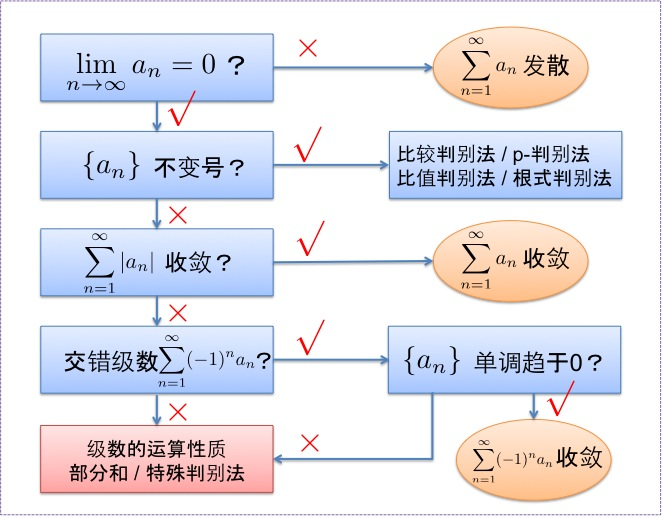
\includegraphics{./images/ch2/seriesCre/010.jpg}}
\end{center}

{\bf 例:}判断正误:
\begin{enumerate}[(1)]
  \setlength{\itemindent}{1cm}
  \item 若$a_n>0(n=1,2,\ldots)$,则\\
  \centerline{$a_1-a_1+a_2-a_2+a_3-a_3+\ldots $}
  收敛 \hfill ({$\times$})
  \item 若以上$\limn a_n=0$,则以上级数收敛 \hfill
  ({$\surd$})
  \item $\sumn a_n$收敛,$\limn b_n=1\Rightarrow\sumn
  a_nb_n$收敛($a_n=\df{(-1)^n}{\sqrt n},b_n=1+a_n$) \hfill ({$\times$})
  \item $\sumn a_n$部分和有界,$\limn b_n=0\Rightarrow\sumn a_nb_n$收敛
  \hfill ({$\times$})
  \item 若$\limn\df{a_n}{b_n}=1$,则若$\sumn a_n$绝对收敛,$\sumn b_n$必收敛 \hfill
  ({$\surd$})
  \item $\sumn a_n,\sumn b_n$绝对收敛$\Rightarrow\sumn (a_n+b_n)$绝对收敛 \hfill
  ({$\surd$})
  \item $\sumn a_n,\sumn b_n$条件收敛$\Rightarrow\sumn (a_n+b_n)$条件收敛 \hfill
  ({$\times$})
  \item 若$\sumn a_n^2$收敛,则$\sumn a_n^3$收敛 \hfill
  ({$\surd$})
\end{enumerate}

{\bf 例:}判断下列级数的敛散性
\begin{enumerate}[(1)]
  \setlength{\itemindent}{1cm}
  
  \item $\df 1{a+b}+\df 1{2a+b}+\df 1{3a+b}+\ldots\quad (a>0,b>0)$
  \item $\sumn\df {a_n}{(1+a_1)(1+a_2)\ldots(1+a_n)}\quad(a_n\geq
	  0,n\in\mathbb{N})$
%   \item $\sumn\df{1!+2!+\ldots+n!}{n!}$
  
%   \item $\sumn\df{\sqrt{n!}}{(2+\sqrt 1)(2+\sqrt 2)\ldots(2+\sqrt n)}$
  \item $\sumn\df{\sqrt{n+1}-\sqrt{n}}{n^p}\quad(p>0)$
  \item $\sumn\df{n^{n+\frac 1{\,n\,}}}{\left(n+\df 1n\right)^n}$\\
  {\bf [hint]:}
  $$a_n=\df{n^{\df1n}}{\left(1+\df1{n^2}\right)^n}\to1\;(n\to\infty)$$
  \item $\sumn\df{2^nn!}{n^n}$
  \item $\sumn n!\left(\df{x}{n}\right)^n\quad (x>0)$\\
  {\bf [hint]:} When $x=e$
  $$\df{a_{n+1}}{a_n}=\df e{\left(1+\df1n\right)^n}>1.$$
  \item $\sumn\left[\df 1n-\ln\left(1+\df 1n\right)\right]$(*)
%   \item $\sumn\df{n^{n+\frac 1{\,n\,}}}{\left(n+\df 1n\right)^n}$
\end{enumerate}

\newpage

blank here

\newpage

\section*{课后作业}

\begin{itemize}
  \item 习题2.1:2,6(1,3),7,9
  \item 已知数列$\{a_n\}$单调递增,它的一个子列$\{a_{n_k}\}$收敛于$a$,
  证明:$\limn a_n=a$。%\\
%   {\bf Pf1:} 由$a_{n_k}\to a(k\to\infty)$,对$\forall\e>0$,$\exists K$,
%   $\forall k>K$,$|a_{n_k}-a|<\e$,或
%   $$a_{n_k}\in U(a,\e).$$
%   令$N=n_{[K]+1}$,则对$\forall n>N$,注意到$\{a_n\}$单调递增,故一定
%   $\exists k>K$,使得$a_na_{n_k}\leq n<a_{n_{k+1}}$,进而
%   $$a_n\in[a_{n_k},a_{n_{k+1}})\subset U(a,\e),$$
%   即证。\\
%   {\bf Pf2:} 由$\{a_n\}$单调递增,对$\forall n\in\mathbb{Z}_+$,
%   $\exists k\in\mathbb{Z}_+$,使得
%   $$a_{n_k}\leq n<a_{n_{k+1}}.$$
%   定义两个数列
%   $$a_n^{(1)}=a_{n_k},\;\mbox{若}a_{n_k}\leq n<a_{n_{k+1}},$$
%   $$a_n^{(2)}=a_{n_{k+1}},\;\mbox{若}a_{n_k}\leq n<a_{n_{k+1}},$$
%   则
%   $$a_n^{(1)}\leq a_n<a_n^{(2)}.$$
%   注意到$\{a_n^{(1)}\},\{a_n^{(2)}\}$的取值范围和$\{a_{n_k}\}$完全相同,
%   且均单调递增,故易知其极限均为$a$。进而,有夹逼定理可知$a_n\to a(n\to\infty)$
  \item 证明:$\sqrt[n]n\to 1\,(n\to\infty)$。
  \item 习题2.2:1(4,6),2(2,3),3,7,9,11
  \item 习题2.3:4,5,6
  \item 写出根植判别法的不等式形式,并证明。
  \item 习题2.4:1,3(3-8),5(2,4),6(1-3),8,9
  \item 习题2.5:2(1,3,6,7,8),3,7,8
\end{itemize}

{\bf 【思考题】}

\begin{itemize}
  \item 习题2.2:6,8,10,12,18
  \item 设$0<a_1<2$,且$(2-a_n)a_{n+1}=1\,(n\in\mathbb{N})$,
  	证明$\{a_n\}$收敛,求其极限。\ps{辅导书(上)-P31-例22}\\
%   {\bf [hint]:} If $a_n=1$, then $a_{n+1}=1$. If $a_n<1$, then $a_{n+1}<1$.
%   If $a_n>2$, then $a_{n+1}<0$, thus $a_{n+2}<\df12$. If $a_n>1$, then 
%   $a_{n+1}>1$. So we have $a_n\in(0,2)$ for sufficient large $n$.\\
%   On the other hand, we have
%   $$a_{n+1}=\df{1-a_{n+1}}{1-a_n}.$$
%   Hence, we can deduce that $a_{n+1}<a_n$, whenever $a_n\in(0,1)$ or 
%   $a_n>1$. So $\{a_n\}$ is mono-increase with upper bound.\\
%   Let $a=\limn a_n$, we can find $a=1$.
  \item 设$x_1=\df 12$,$x_{n+1}=x_n^2+x_n\,(n\in\mathbb{N})$,求
	$$\limn\left(\df 1{x_1+1}+\df 1{x_2+1}+\ldots+\df
	1{x_n+1}\right)$$
%   {\bf [hint]:}$\df1{x_{n+1}}=\df1{x_n}-\df1{x_n+1}$, so we have
%   $$\df1{x_n+1}=\df1{x_n}-\df1{x_{n+1}}$$
  \item 已知$0<x<1$,数列$\{a_n\}$定义如下:
	$$a_1=\df x2,\;a_n=\df x2-\df{a_{n-1}^2}2.$$
	证明$\{a_n\}$收敛,并求其极限。
  \item 已知$0<x<1$,数列$\{a_n\}$定义如下:\ps{参考辅导书(上)-P30-例21}
	$$a_1=\df x2,\;a_n=\df x2+\df{a_{n-1}^2}2.$$
	证明$\{a_n\}$收敛,并求其极限。
% 	\ps{参考辅导书(上)-P30-例21,是不是题目抄错了?应该是$\df x2+\df{a_{n-1}^2}2$}\\
%   {\bf [hint]:} It's easy to find $a_2\in(0,a_1)$. Assume $a_{n}\in
%   (0,a_{n-1})$, then
%   $$a_n=\df x2-\df{a_{n-1}^2}2<\df x2-\df{a_{n}^2}2=a_{n+1}.$$
%   We can find $\limn a_n=\sqrt{x+1}-1$.  
  \item 习题2.3:7,8 
  \item 习题2.4:10-15,17
  \item 习题2.5:4,6,10,13
\end{itemize}
% 
% \newpage
% 
% $$\df1{x^3(1+x^4)}=\df{Ax^2+Bx+C}{x^3}+\df{Dx^3+Ex^2+Fx+G}{1+x^4}$$

\newpage

{\bf 命题:}若$\{a_n\}$有界,且$\{a_n-a_{n-1}\}$收敛于$0$,则$\{a_n\}$收敛。

{\bf 反例:}

(1)$\sin\sqrt n$

(2)$\left\{\left(\sum\limits_{k=1}^n\df1k\right)\mod
2-1\right\}(-1)^{\left[\frac12{\sum\limits_{k=1}^n\frac1k}\right]}$

{\bf 例:}已知$0<x<1$,数列$\{a_n\}$定义如下:
$$a_1=\df x2,\;a_n=\df x2-\df{a_{n-1}^2}2.$$
证明$\{a_n\}$收敛,并求其极限。

{\bf 证}: 若极限存在,易求得$\limn a_n=1+\sqrt{1+x}$。以下证明$\{a_n\}$收敛。

显然$x_n\in\left(0,\df x2\right),(n\in\mathbb Z_+)$。由递推公式可得

% 显然,$x_n<\df x2\;(n\in\mathbb{Z}_+)$。
% \begin{align}
% 	a_n-a_{n-1}&=-\df12(a_{n-1}-a_{n-2})(a_{n-1}+a_{n-2})\notag\\
% 	&=\left(-\df12\right)^2(a_{n-2}-a_{n-3})(a_{n-2}+a_{n-3})(a_{n-1}+a_{n-2})\notag\\
% 	&=\ldots=\left(-\df12\right)^{n-2}(a_2-a_1)(a_2+a_1)\ldots
% 	(a_{n-2}+a_{n-3})(a_{n-1}+a_{n-2})\notag
% \end{align}
% 注意到对任意$n\in\mathbb{Z}_+$
% $$a_n+a_{n-1}=\df{1+x}2-\df12(a_n-1)^2<\df{1+x}2<1,$$
% 故有
% $$|a_n-a_{n-1}|<|a_2-a_1|\left(\df{1+x}4\right)^{n-2}\to0,
% \;(n\to\infty)$$

$$a_n-a_{n-1}=-\df12(a_{n-1}-a_{n-2})(a_{n-1}+a_{n-2}),$$
由此可知若$a_{n-1}>a_{n-2}$,则$a_n<a_{n-1}$。又
$$a_n+a_{n-1}=\df{1+x}2-\df12(a_n-1)^2<\df{1+x}2<1,$$
故
$$|a_n-a_{n-1}|<\df12|a_{n-1}-a_{n-2}|.$$
从而,若$a_{n-1}>a_{n-2}$,则必有$a_{n-2}<a_n<a_{n-1}$,进而
可以证明$a_n<a_{n+1}<a_{n-1}$,也即$[a_n,a_{n+1}]\subset[a_{n-2},a_{n-1}]$。
注意到$x_2<x_1$,故可以断言$\{a_n\}$的偶子列和奇子列分别是单调递增
和单调递减的,从而区间序列$\{[a_{2n},a_{2n-1}]\}$构成了一个区间套,也即
$$[a_{2n+2},a_{2n+1}]\subset[a_{2n},a_{2n-1}],\;(n\in\mathbb Z_+).$$

另一方面,由
\begin{align}
	a_n-a_{n-1}&=-\df12(a_{n-1}-a_{n-2})(a_{n-1}+a_{n-2})\notag\\
	&=\left(-\df12\right)^2(a_{n-2}-a_{n-3})(a_{n-2}+a_{n-3})(a_{n-1}+a_{n-2})\notag\\
	&=\ldots=\left(-\df12\right)^{n-2}(a_2-a_1)(a_2+a_1)\ldots
	(a_{n-2}+a_{n-3})(a_{n-1}+a_{n-2}),\notag
\end{align}
可得
$$|a_n-a_{n-1}|<|a_2-a_1|\left(\df{1+x}4\right)^{n-2}\to0,
\;(n\to\infty),$$
从而必有$\limn(a_n-a_{n-1})=0$,进而$\limn(a_{2n}-a_{2n-1})=0$。

综上,区间序列$\{[a_{2n},a_{2n-1}]\}$满足区间套定理(习题2.2-12)条件,
从而$\{a_{2n}\}$和$\{a_{2n-1}\}$收敛于相同的极限,由拉链定理,$\{a_n\}$收敛。

\newpage

{\bf 例:}设$\limn a_n=a>0$,判断级数$\sumn\left(\df{a}{a_n}\right)^n$
的敛散性

[hint]:由条件不能判定!

(1)若$a_n=a$,显然级数发散。

(2)设$a_n=\df{1+\sqrt n}{\sqrt n}\to1=a(n\to\infty)$,则
$$\sumn\left(\df{a}{a_n}\right)^n=\sumn\left(\df{\sqrt n}
{1+\sqrt n}\right)^n,$$
由对数判别法
$$-\limn\df{\ln \left(\df{\sqrt n}{1+\sqrt n}\right)^n}
{\ln n}=\limn\df{n[\ln(\sqrt n+1)-\ln\sqrt n]}{\ln n}
=\limn\df{\sqrt n}{\ln n}=+\infty>1,$$
故级数收敛。
